\documentclass{article}
\usepackage{graphicx}
\graphicspath{ {.} }

\begin{document}

The algorithm finds whether a number is a leap year or not in a rather straightforward manner - it checks the conditions for a year being a leap year one at a time.
The conditions are arranged such that the overlap between them is taken into account. 
E.g. the condition that the year is divisible by 400 has to come before the 'divisible by 100' condition, else it might reach a case where both are conditions true, but 'false' is returned, which would be incorrect.
The console part of the application is also included in the illustration - user input which is not a valid number simply returns 'nay' instead of throwing an exception.


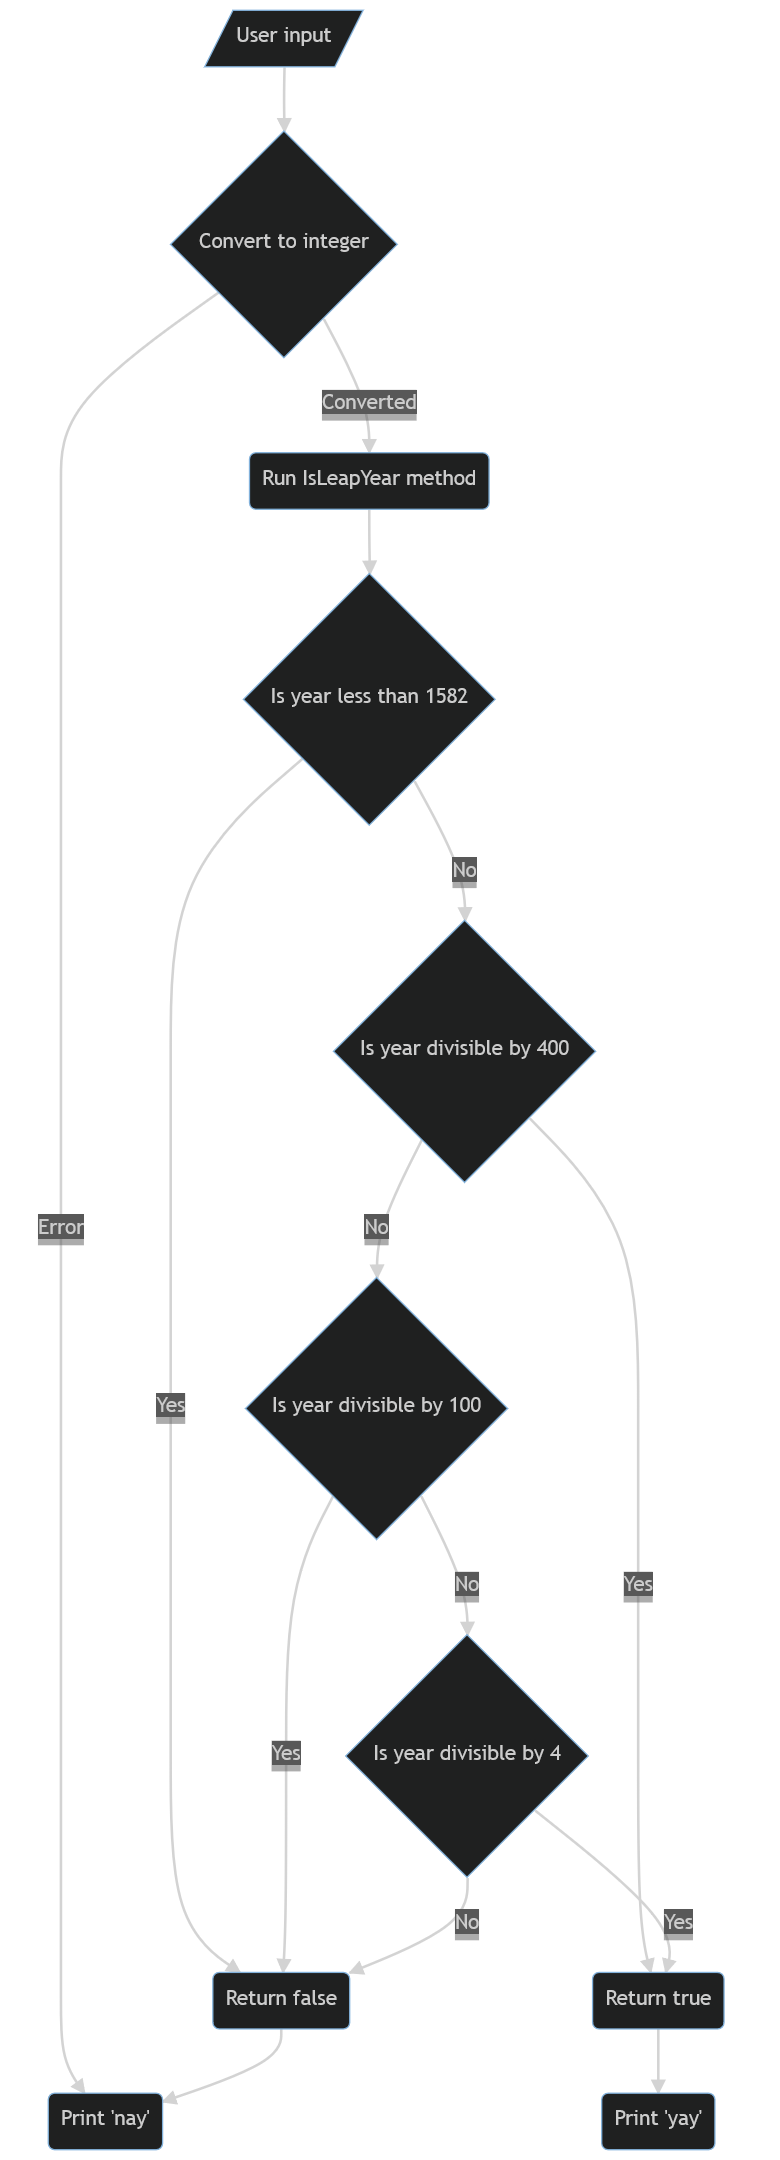
\includegraphics[width=\textwidth,height=\textheight,keepaspectratio]{diagram.png}


\end{document}